%%%%%%%%%%%%%%%%%%%%%%%%%%%%%%%%%%%%%%%%%
% Beamer Presentation
% LaTeX Template
% Version 1.0 (10/11/12)
%
% This template has been downloaded from:
% http://www.LaTeXTemplates.com
%
% License:
% CC BY-NC-SA 3.0 (http://creativecommons.org/licenses/by-nc-sa/3.0/)
%
%%%%%%%%%%%%%%%%%%%%%%%%%%%%%%%%%%%%%%%%%

%----------------------------------------------------------------------------------------
%	PACKAGES AND THEMES
%----------------------------------------------------------------------------------------

%\documentclass{beamer}
\documentclass[12pt, aspectratio=169]{beamer}
\usepackage{keynote-gradient-white}

\mode<presentation> {

% The Beamer class comes with a number of default slide themes
% which change the colors and layouts of slides. Below this is a list
% of all the themes, uncomment each in turn to see what they look like.

%\usetheme{default}
%\usetheme{AnnArbor}
%\usetheme{Antibes}
%\usetheme{Bergen}
%\usetheme{Berkeley}
%\usetheme{Berlin}
%\usetheme{Boadilla}
%\usetheme{CambridgeUS}
%\usetheme{Copenhagen}
%\usetheme{Darmstadt}
%\usetheme{Dresden}
%\usetheme{Frankfurt}
%\usetheme{Goettingen}
%\usetheme{Hannover}
%\usetheme{Ilmenau}
%\usetheme{JuanLesPins}
%\usetheme{Luebeck}
%\usetheme{Madrid}
%\usetheme{Malmoe}
%\usetheme{Marburg}
%\usetheme{Montpellier}
%\usetheme{PaloAlto}
%\usetheme{Pittsburgh}
%\usetheme{Rochester}
%\usetheme{Singapore}
%\usetheme{Szeged}
%\usetheme{Warsaw}

% As well as themes, the Beamer class has a number of color themes
% for any slide theme. Uncomment each of these in turn to see how it
% changes the colors of your current slide theme.

%\usecolortheme{albatross}
%\usecolortheme{beaver}
%\usecolortheme{beetle}
%\usecolortheme{crane}
%\usecolortheme{dolphin}
%\usecolortheme{dove}
%\usecolortheme{fly}
%\usecolortheme{lily}
%\usecolortheme{orchid}
%\usecolortheme{rose}
%\usecolortheme{seagull}
%\usecolortheme{seahorse}
%\usecolortheme{whale}
%\usecolortheme{wolverine}

%\setbeamertemplate{footline} % To remove the footer line in all slides uncomment this line
%\setbeamertemplate{footline}[page number] % To replace the footer line in all slides with a simple slide count uncomment this line

%\setbeamertemplate{navigation symbols}{} % To remove the navigation symbols from the bottom of all slides uncomment this line
}

\usepackage{graphicx} % Allows including images
\usepackage{booktabs} % Allows the use of \toprule, \midrule and \bottomrule in tables
\usepackage{hyperref}

%--------------------------------------------------------------------------------
%	TITLE PAGE
%--------------------------------------------------------------------------------

\title[Neurotechnologies to manage a robotic system]{Neurotechnologies to manage a robotic system} % The short title appears at the bottom of every slide, the full title is only on the title page

\author[Max Talanov]{
  % 
\includegraphics[height=2cm]{ITIS_logo_bright}\\
  Max Talanov
} 
\institute[NcN laboratory: ITIS : KFU]% Your institution as it will appear on the bottom of every slide, may be shorthand to save space
{
Neuromorphic computing and Neurosimulations laboratory, ITIS, KFU \\ % Your institution for the title page
\medskip
\textit{max.talanov@gmail.com} % Your email address
}
\date{\today} % Date, can be changed to a custom date

\begin{document}

\begin{frame}
\titlepage % Print the title page as the first slide
\end{frame}


%-------------------------------------------------------------------------------
% Neural network
%-------------------------------------------------------------------------------

%------------------------------------------------
\section{Neural network}

%------------------------------------------------
\begin{frame}
  \frametitle{Convolutional neural network}
  \begin{figure}
    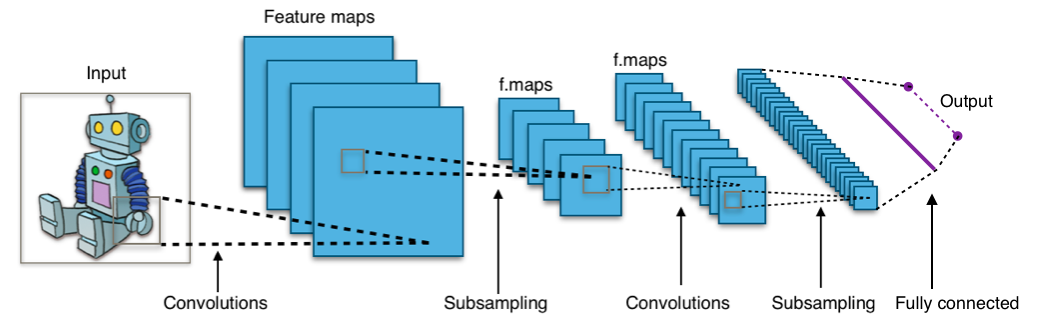
\includegraphics[width=0.9\linewidth]{Typical_cnn}
  \end{figure}
  \footnotetext{\url{https://en.wikipedia.org/wiki/Convolutional_neural_network}}
\end{frame}

%------------------------------------------------


%------------------------------------------------
\begin{frame}
  \frametitle{ResNet}
  \begin{columns}
    \begin{column}{0.45\textwidth}
      \begin{figure}
        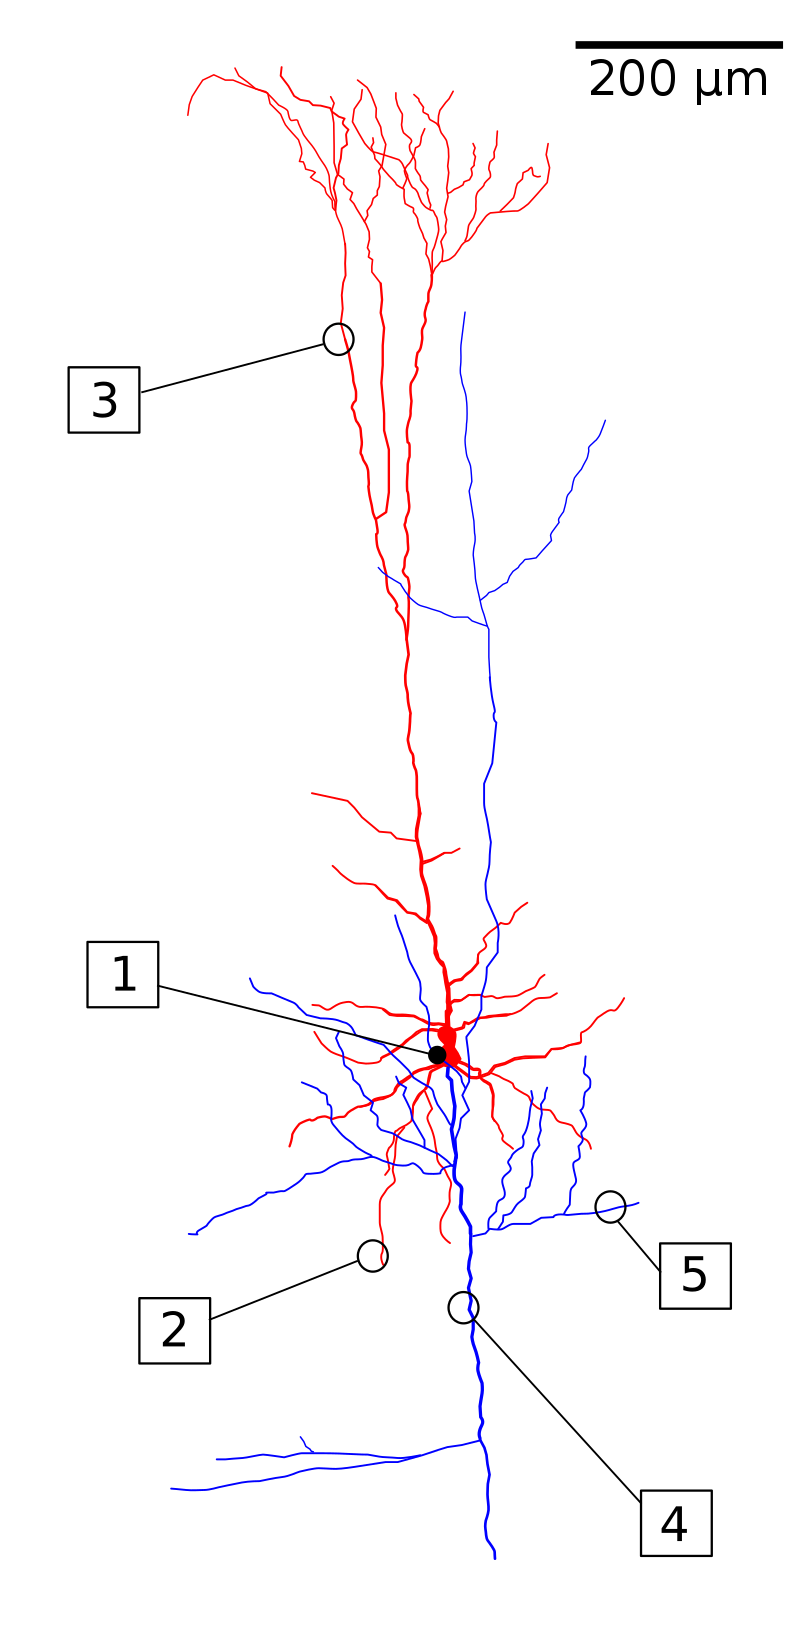
\includegraphics[width=0.45\linewidth]{800px-Piramidal_cell.svg}
      \end{figure}
    \end{column}
    \begin{column}{0.55\textwidth}
      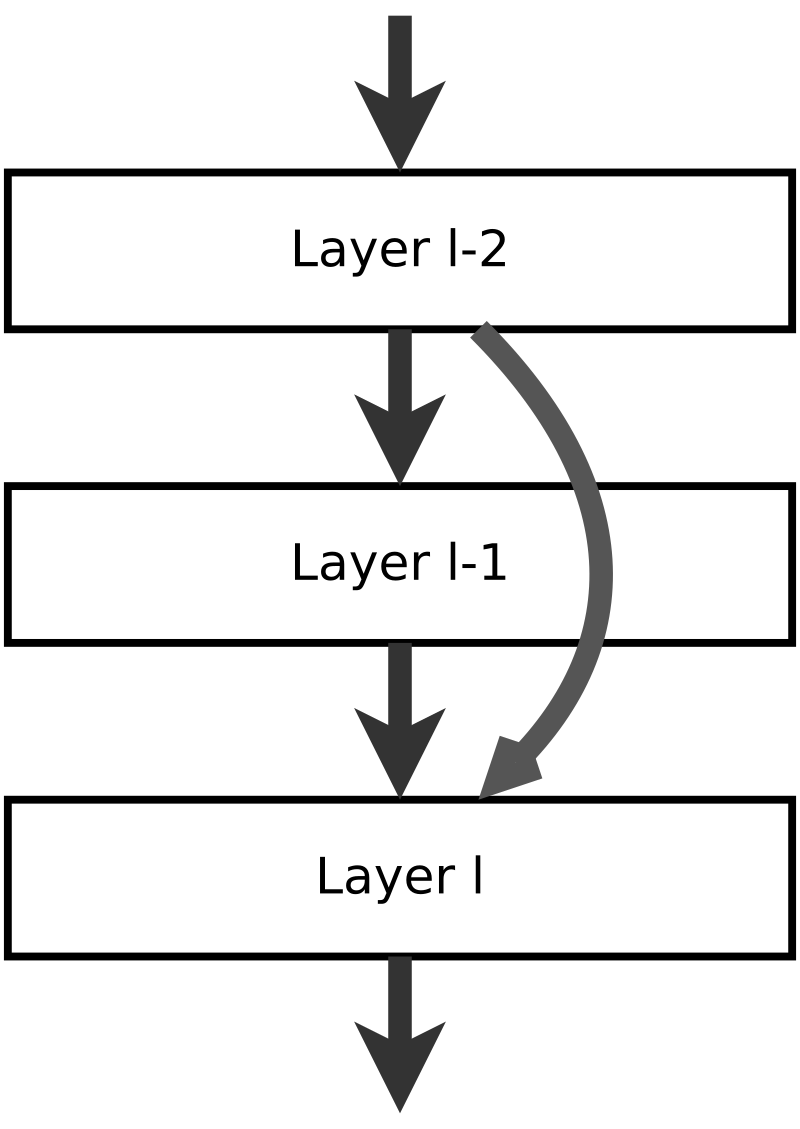
\includegraphics[width=0.55\textwidth]{800px-ResNets.svg}
    \end{column}
  \end{columns}
  \footnotetext{\url{https://en.wikipedia.org/wiki/Residual_neural_network}}
\end{frame}


%-------------------------------------------------------------------------------
% Kevin Warwick
%-------------------------------------------------------------------------------

%------------------------------------------------
\section{Kevin Warwick}
%------------------------------------------------
\begin{frame}
  \frametitle{Kevin Warwick fist cyborg}
  \begin{figure}
    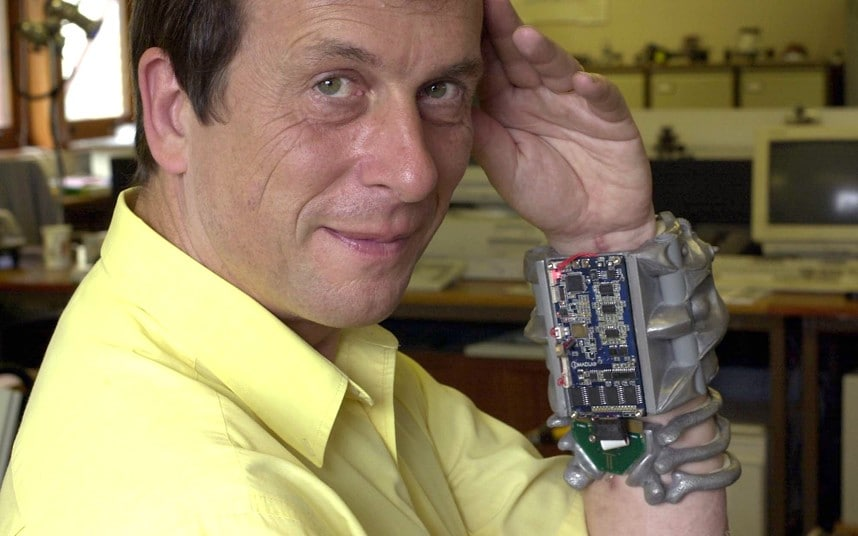
\includegraphics[width=0.7\linewidth]{Kevin-Warwick_2936650k}
  \end{figure}
  \footnotetext{\url{https://www.telegraph.co.uk/}}
\end{frame}

%------------------------------------------------

%------------------------------------------------
\begin{frame}
  \frametitle{Utah array}
  \begin{figure}
    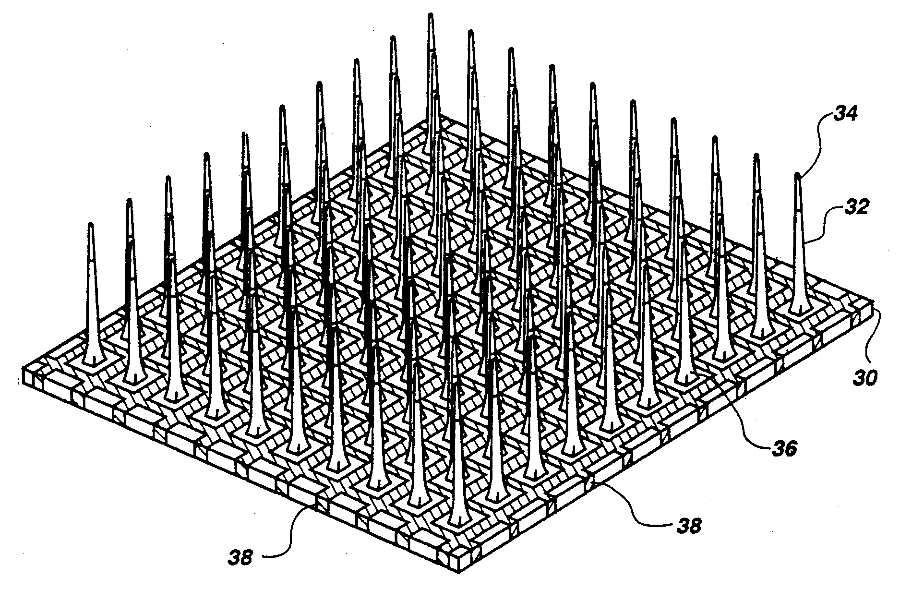
\includegraphics[width=0.7\linewidth]{Utah_array_pat5215088}
  \end{figure}
  \footnotetext{\url{https://en.wikipedia.org/wiki/Microelectrode_array}}
\end{frame}

%------------------------------------------------

%------------------------------------------------
\begin{frame}
  \frametitle{Robot managed by rat brain}
  \begin{figure}
    \includegraphics[width=0.33\linewidth]{Miabot}
  \end{figure}
  \footnotetext{\url{https://www.dailymail.co.uk/sciencetech/}}
\end{frame}

%------------------------------------------------


%-------------------------------------------------------------------------------
% Nicolelis and Lebedev
%-------------------------------------------------------------------------------

%------------------------------------------------
\section{Nicolelis and Lebedev}
%------------------------------------------------
\begin{frame}
  \frametitle{Nicolelis \& Lebedev}
  \begin{figure}
    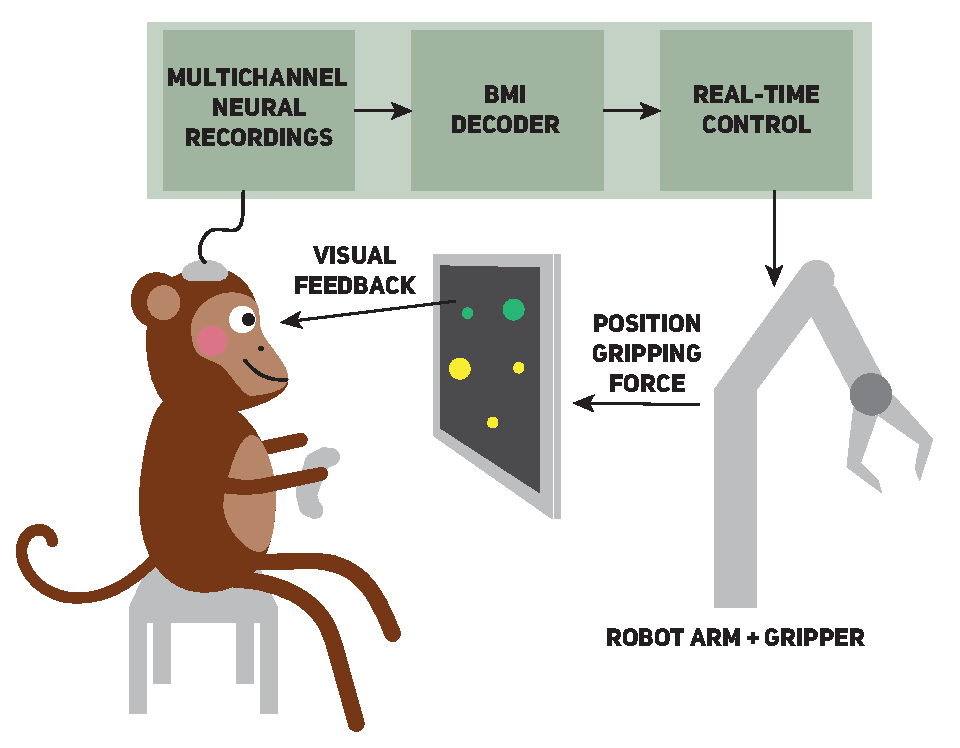
\includegraphics[width=0.6\linewidth]{monkey}
  \end{figure}
  \footnotetext{adopted from Mikhail A. Lebedev and Miguel A. L. Nicolelis, Brain-Machine Interfaces: From Basic Science to Neuroprostheses and Neurorehabilitation}
\end{frame}

%------------------------------------------------

%-------------------------------------------------------------------------------
% Neuralink
%-------------------------------------------------------------------------------

%------------------------------------------------
\section{Neuralink}

%------------------------------------------------
\begin{frame}
  \frametitle{Neuralink: Musk presenting link interface}
  \begin{figure}
    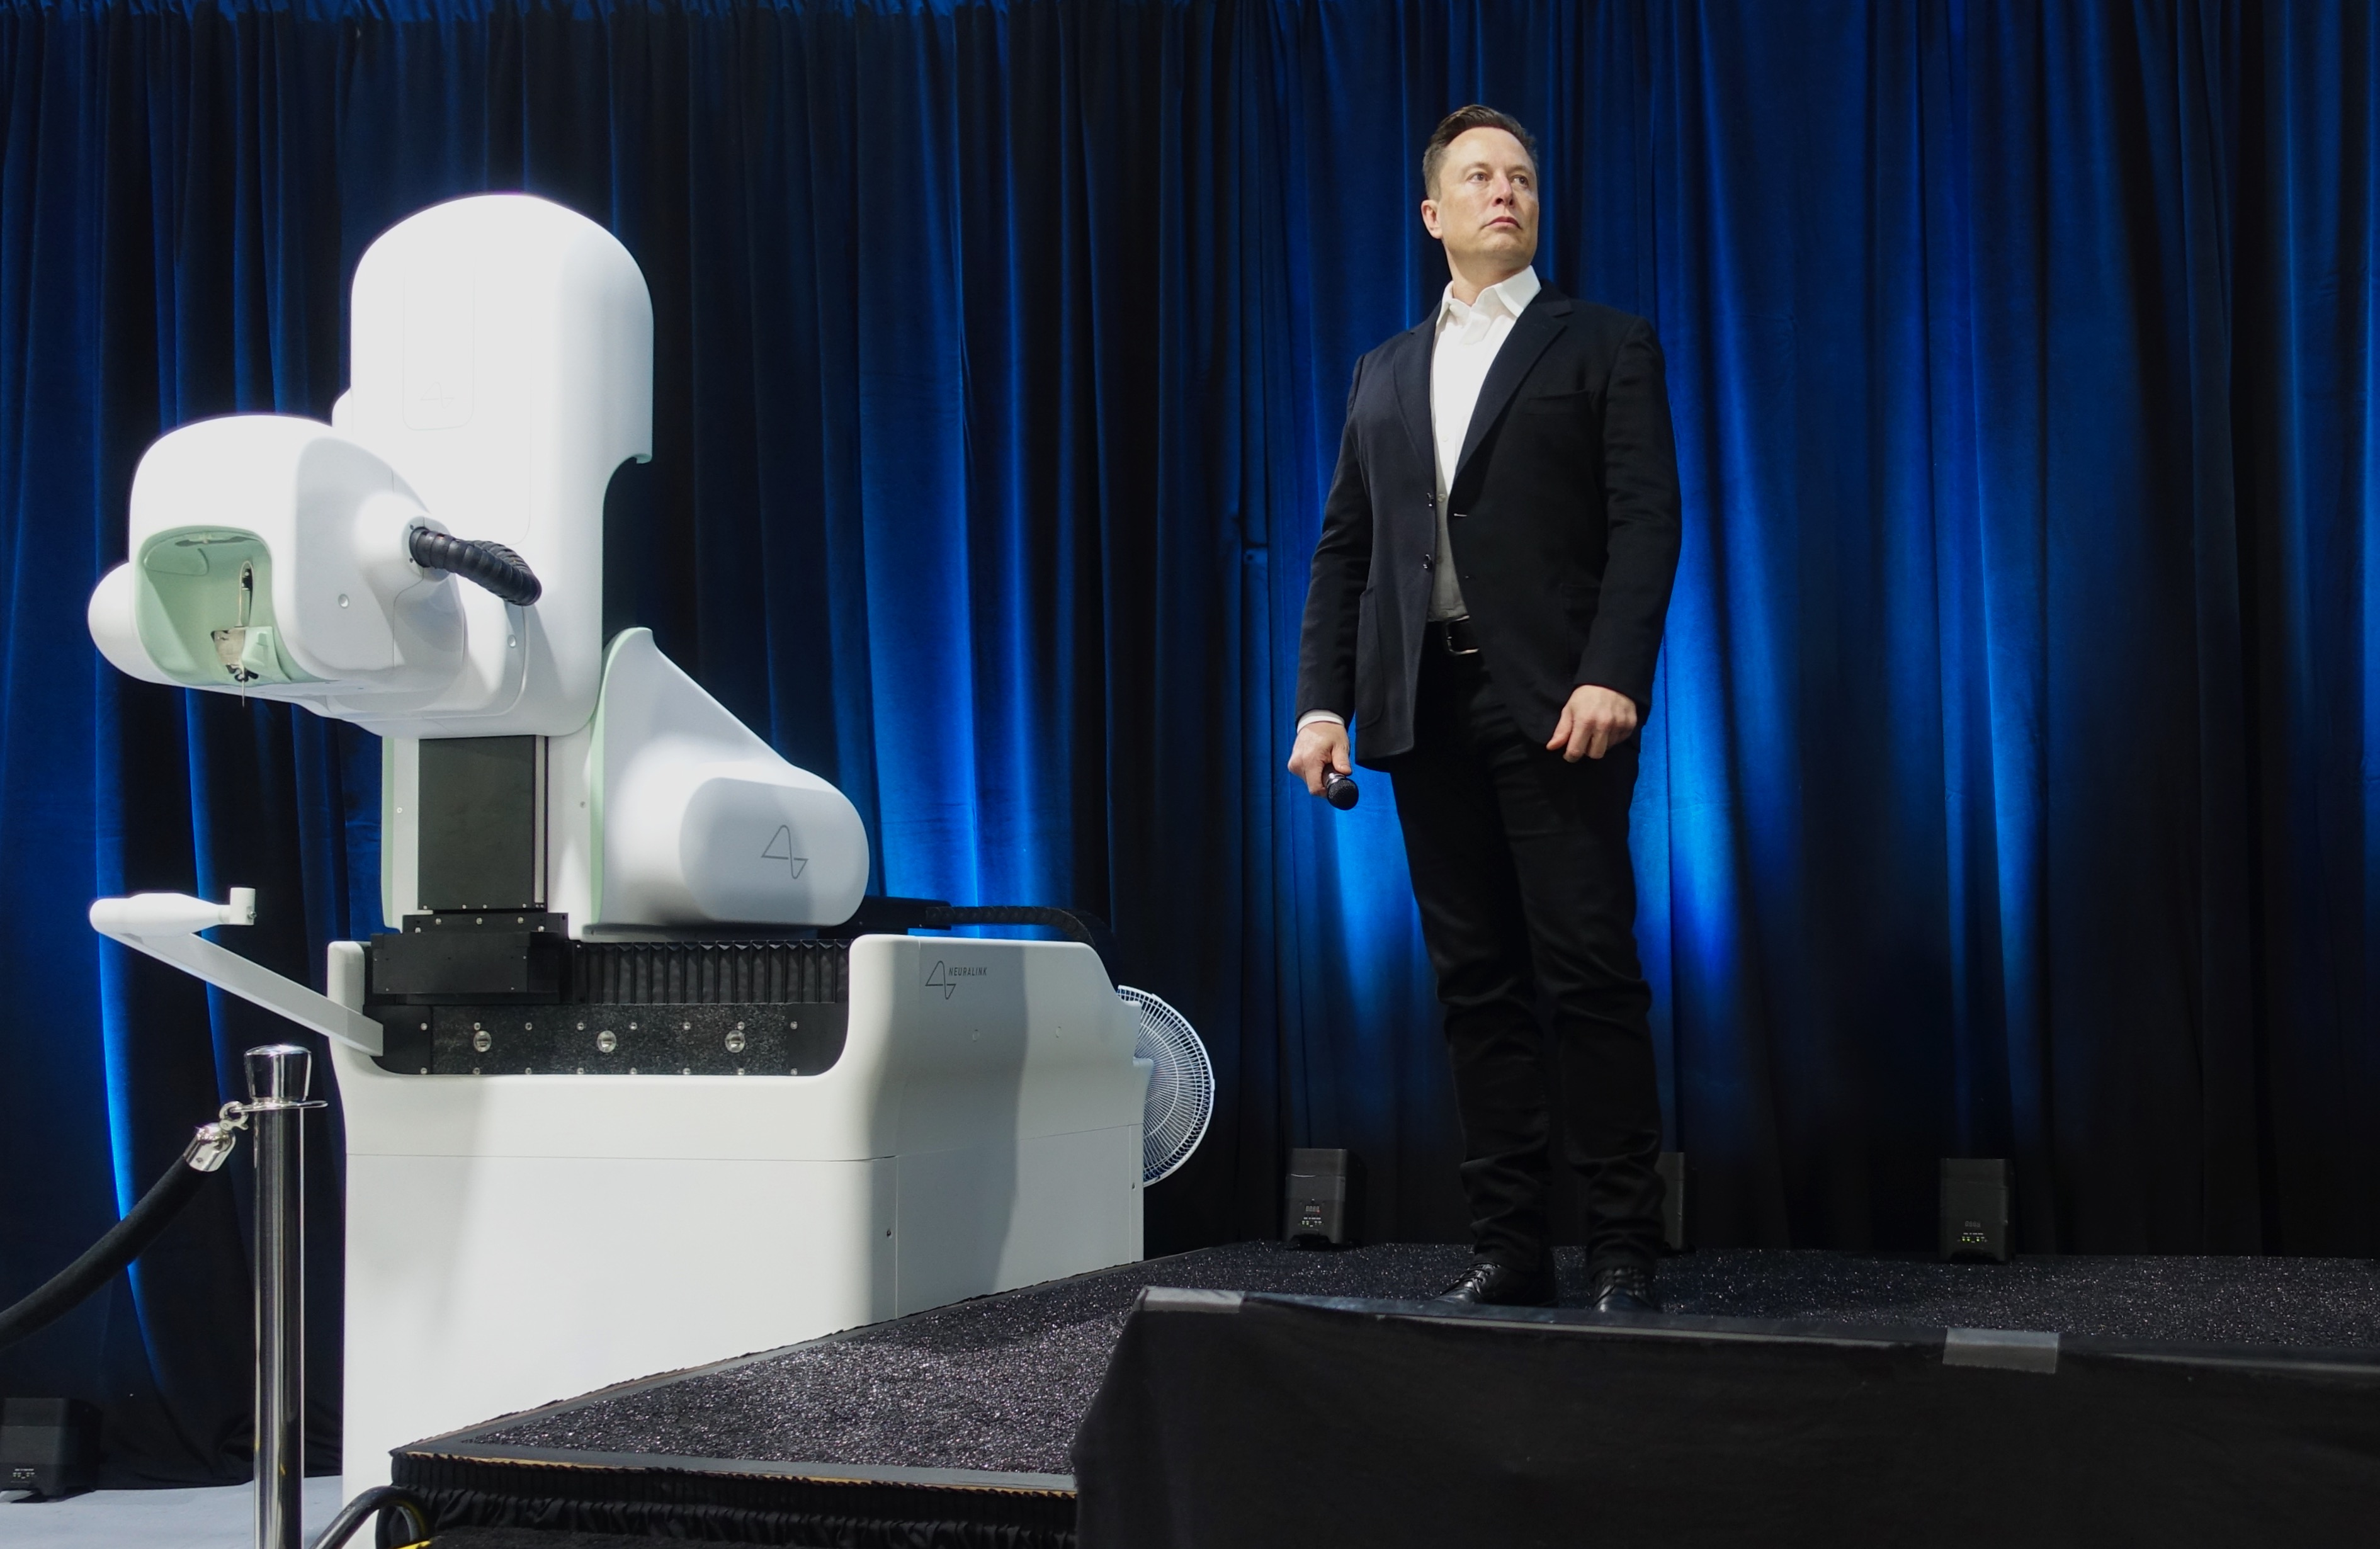
\includegraphics[width=0.6\linewidth]{Elon_Musk_and_the_Neuralink_Future}
  \end{figure}
  \footnotetext{https://en.wikipedia.org/wiki/Neuralink}
\end{frame}

%------------------------------------------------

%------------------------------------------------
\begin{frame}
  \frametitle{Neuralink: link interface}
  \begin{figure}
    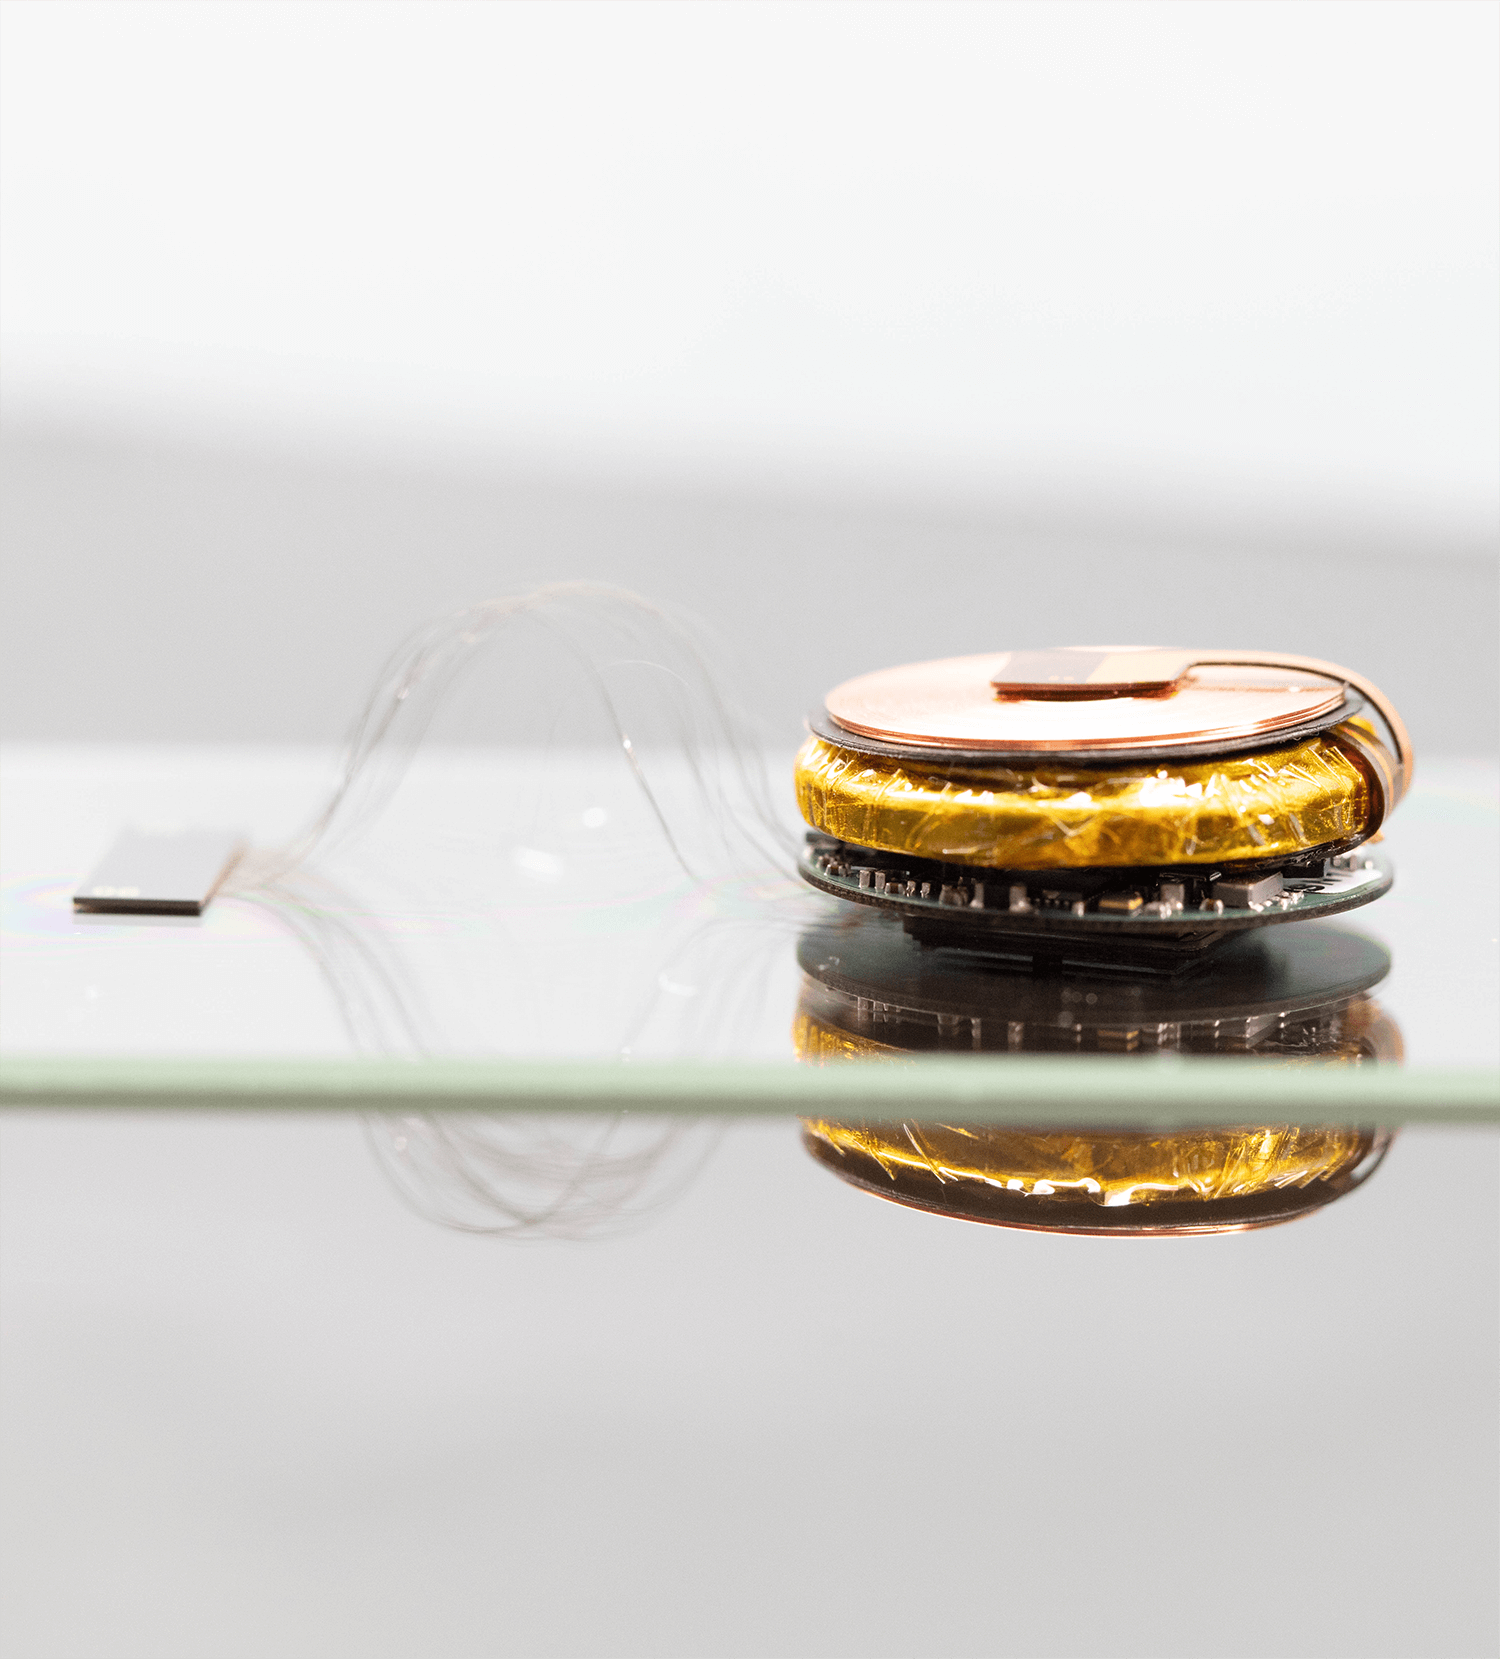
\includegraphics[width=0.4\linewidth]{approach-link-1}
  \end{figure}
  \footnotetext{https://neuralink.com/approach/}
\end{frame}

%------------------------------------------------


%-------------------------------------------------------------------------------
% Memristive spinal cord
%-------------------------------------------------------------------------------

%------------------------------------------------
\section{The problem (current state of cutting edge neuro-rehabilitation technology)}
%------------------------------------------------
\begin{frame}
  \frametitle{Neuro-rehabilitation: Epidural stimulation}
  \begin{figure}
    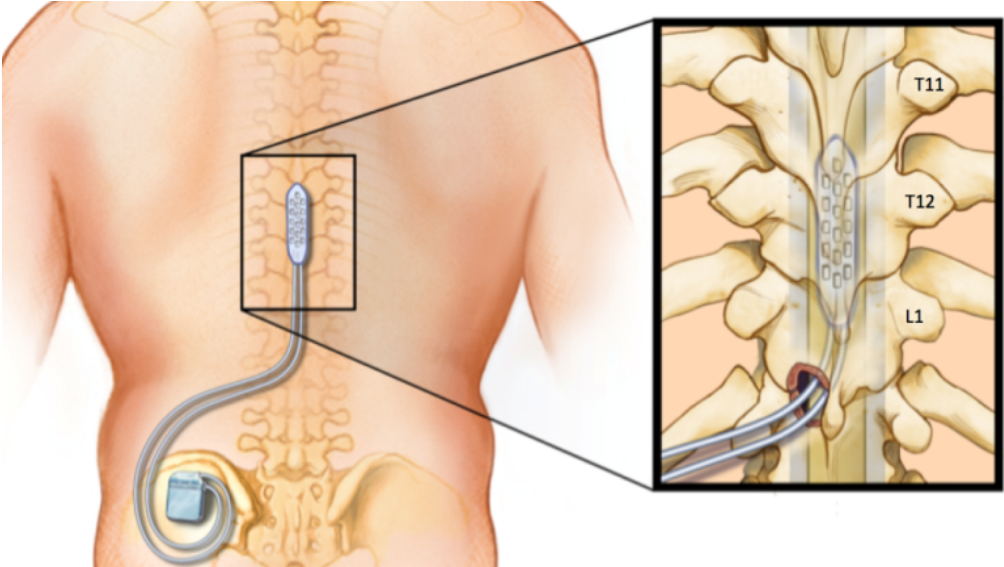
\includegraphics[width=0.6\linewidth]{epidural_stimulation_spinal_cord}
  \end{figure}
\end{frame}

%------------------------------------------------
\begin{frame}
  \frametitle{Neuro-rehabilitation}
  \begin{figure}
    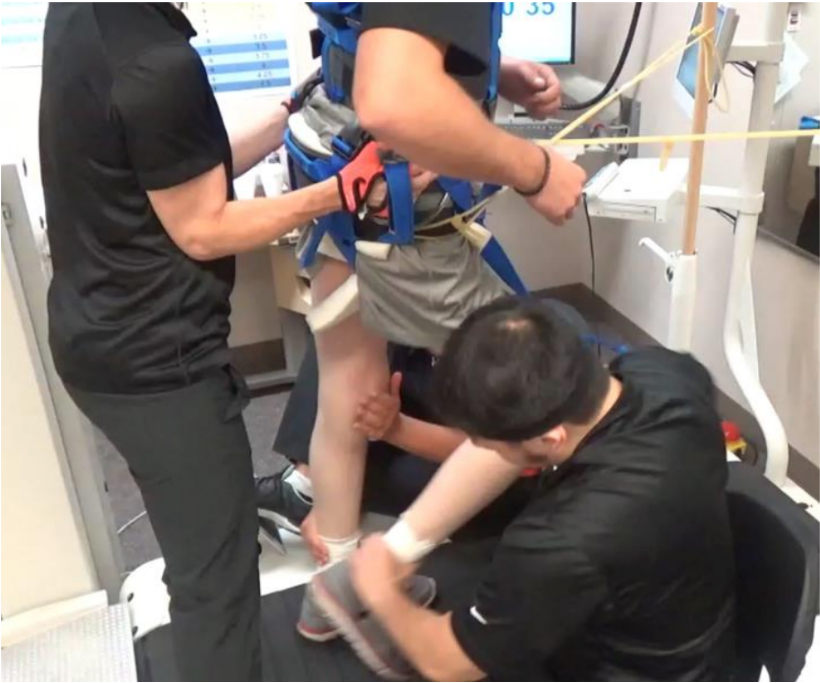
\includegraphics[width=0.5\linewidth]{neurorehabilitation}
  \end{figure}
\end{frame}

%------------------------------------------------
\section{Solution - Igor Lavrov model}
%------------------------------------------------
\begin{frame}
  \frametitle{Model of Lavrov}
  \begin{figure}
    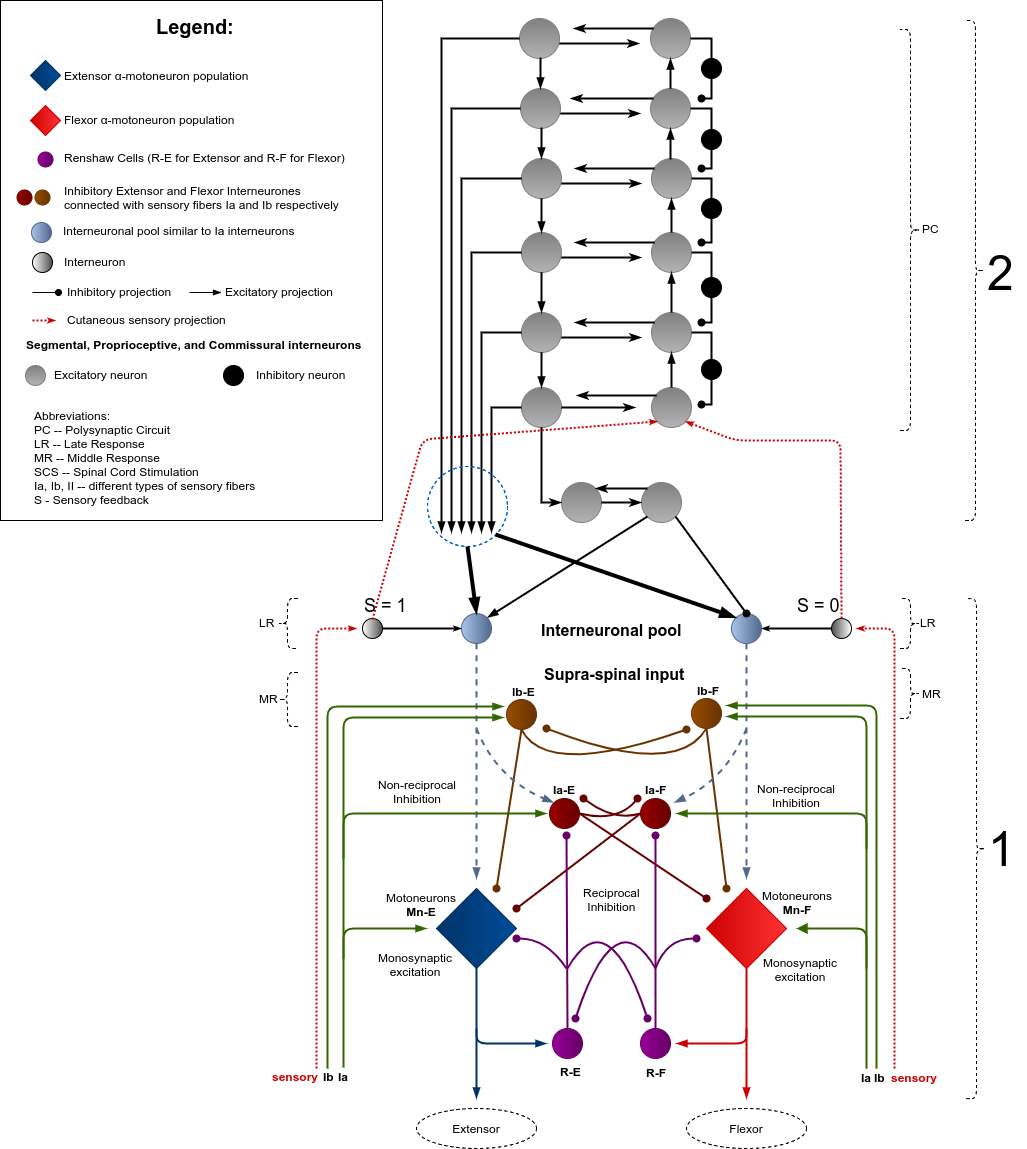
\includegraphics[width=0.48\linewidth]{spinal-cord-diagram}
  \end{figure}
\end{frame}
%------------------------------------------------
\subsection{Neuro-simulation results}
%------------------------------------------------
\begin{frame}
  \frametitle{Simulation results compared with bio results}
  \begin{figure}
    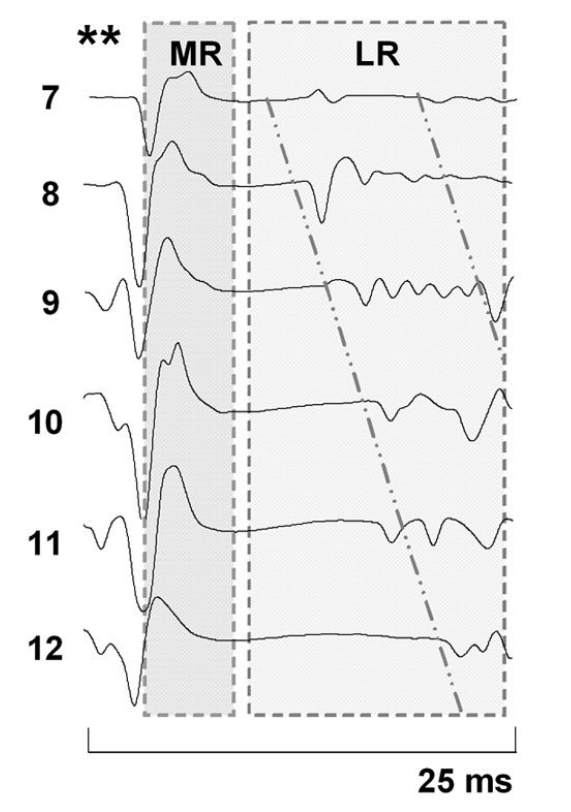
\includegraphics[width=0.2725\linewidth]{mscs_biological_results}
    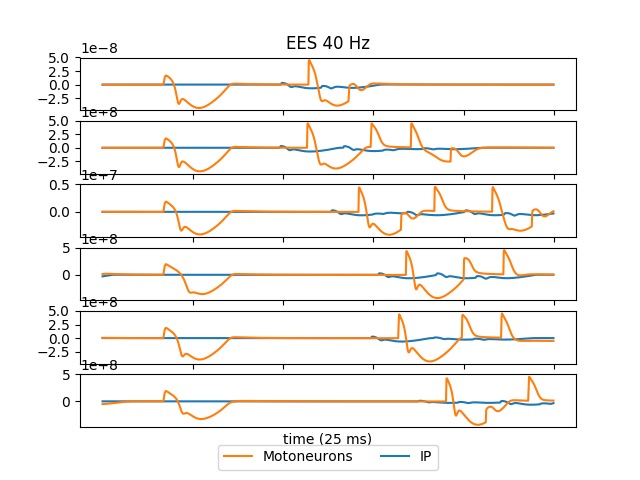
\includegraphics[width=0.60\linewidth]{cpg_40Hz_100p}
  \end{figure}
\end{frame}

%------------------------------------------------

%------------------------------------------------
\section{Even simpler real-time model of neuron}
%------------------------------------------------
\begin{frame}
  \frametitle{ESRN}
  \begin{figure}
    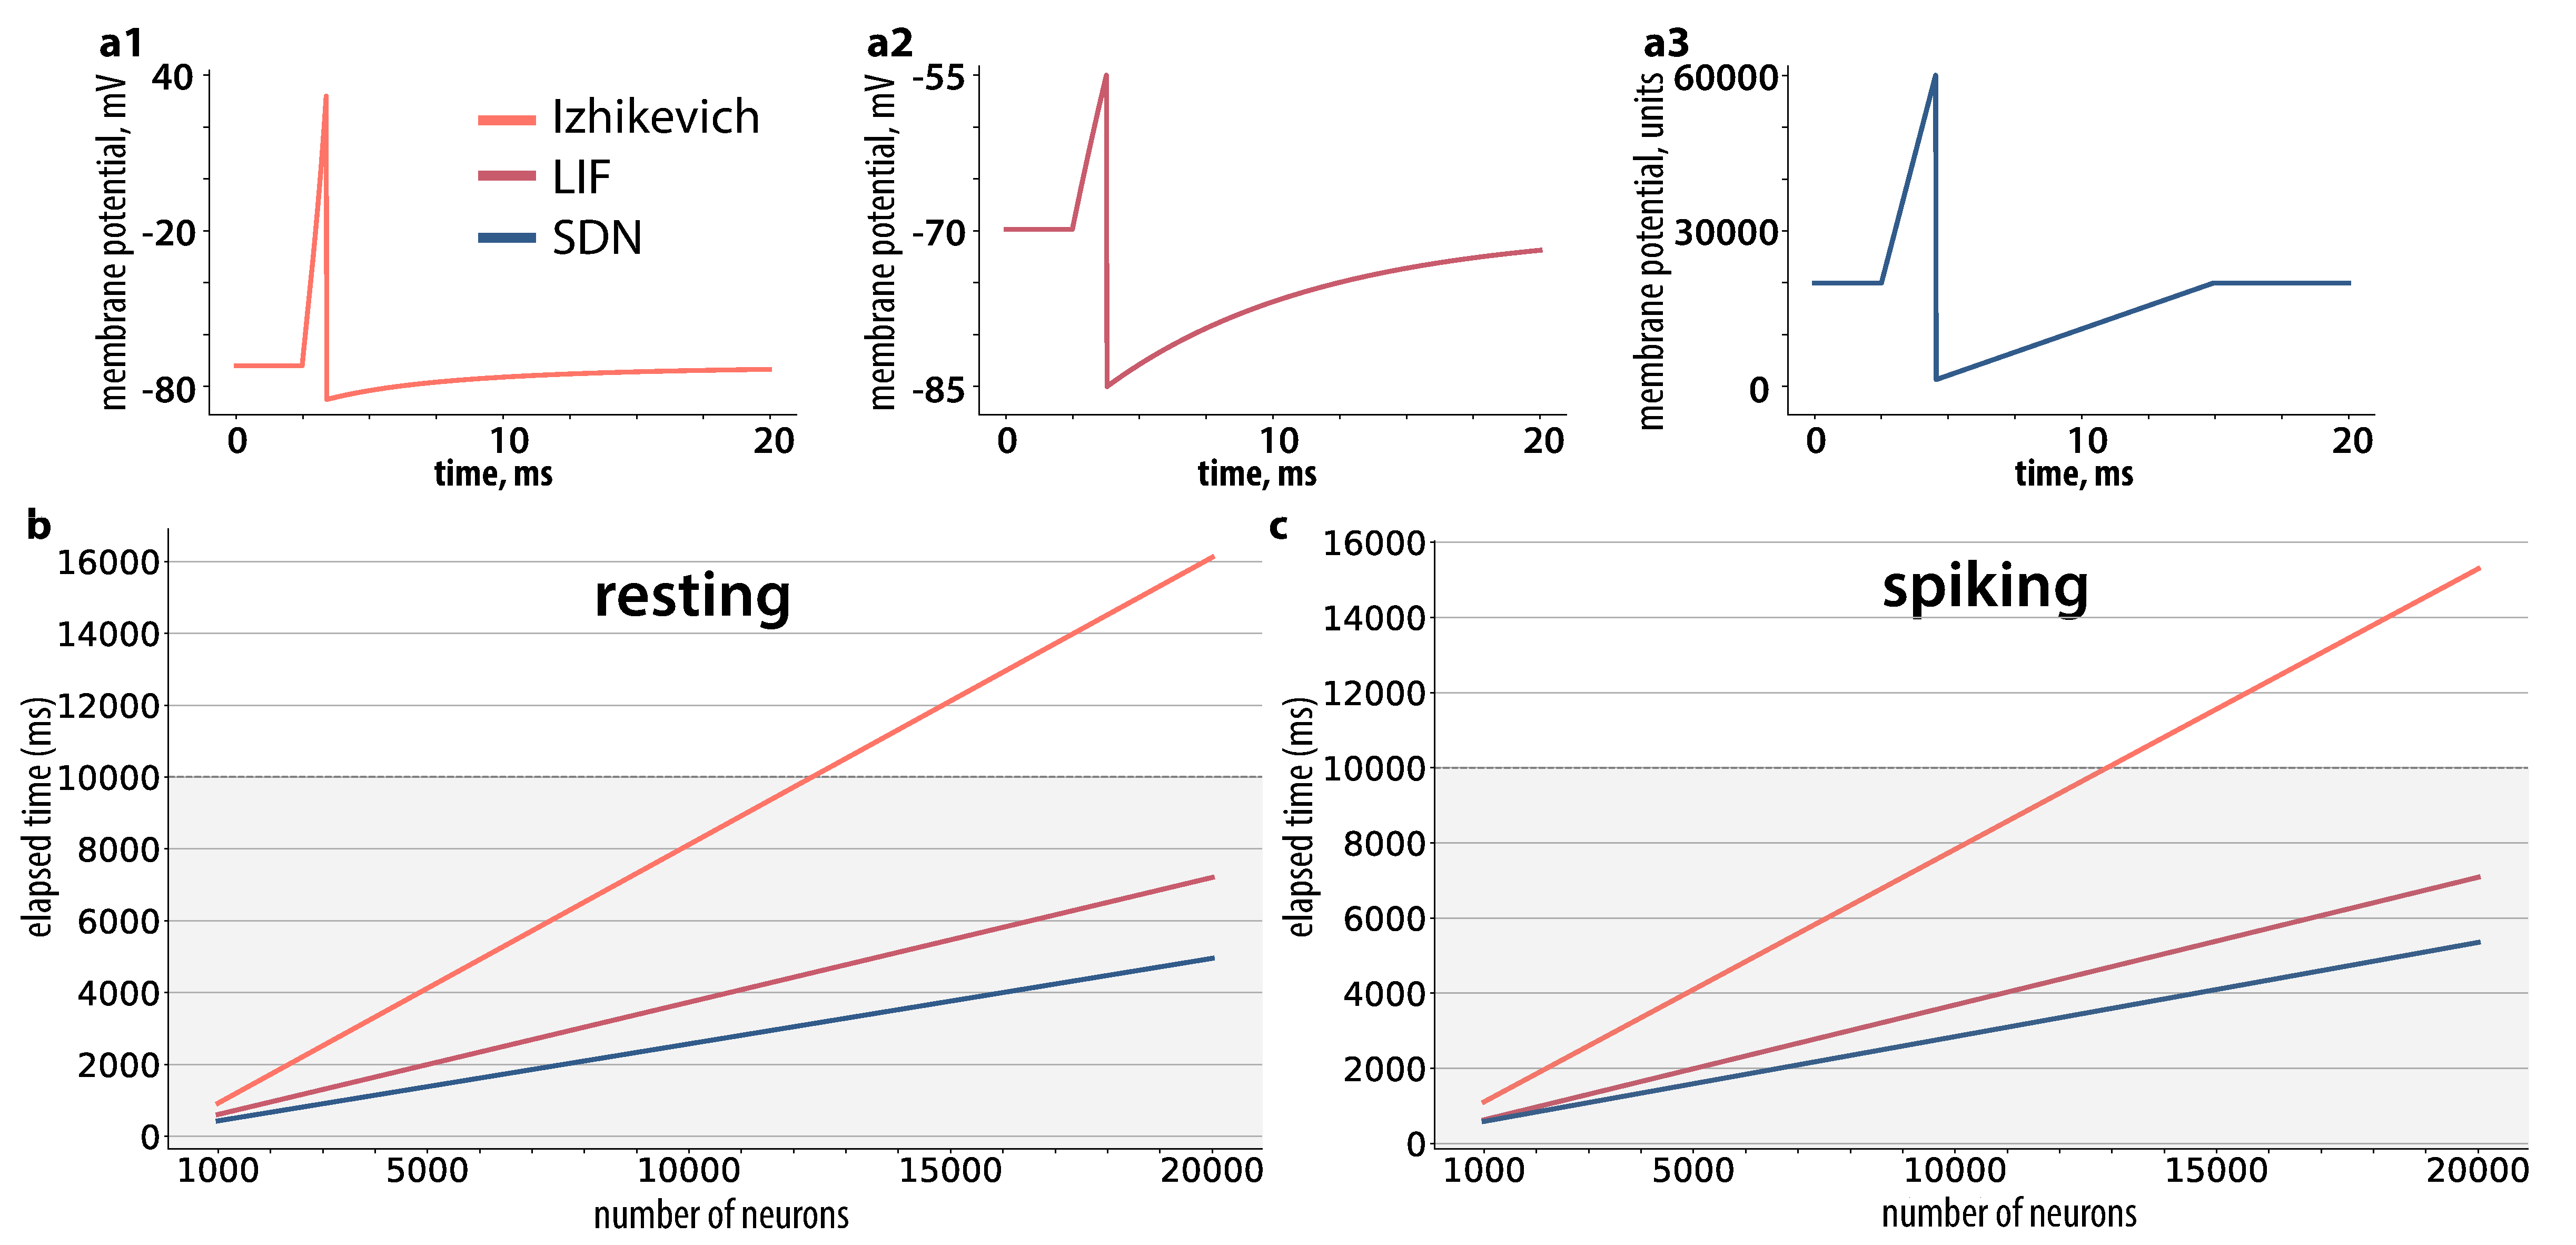
\includegraphics[width=0.8\linewidth]{states}
  \end{figure}
\end{frame}
%------------------------------------------------

%------------------------------------------------
\section{Oscillator motif}
%------------------------------------------------
\begin{frame}
  \frametitle{Oscillator motif}
  \begin{figure}
    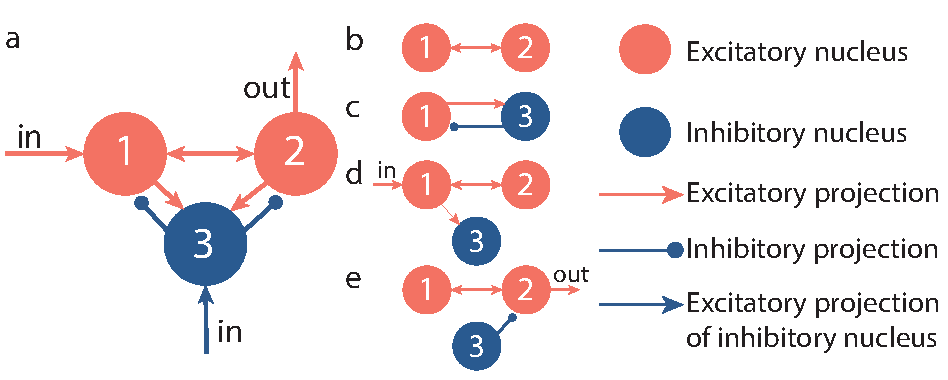
\includegraphics[width=0.8\linewidth]{OM}
  \end{figure}
\end{frame}
%------------------------------------------------
\begin{frame}
  \frametitle{Oscillator motif simulation}
  \begin{figure}
    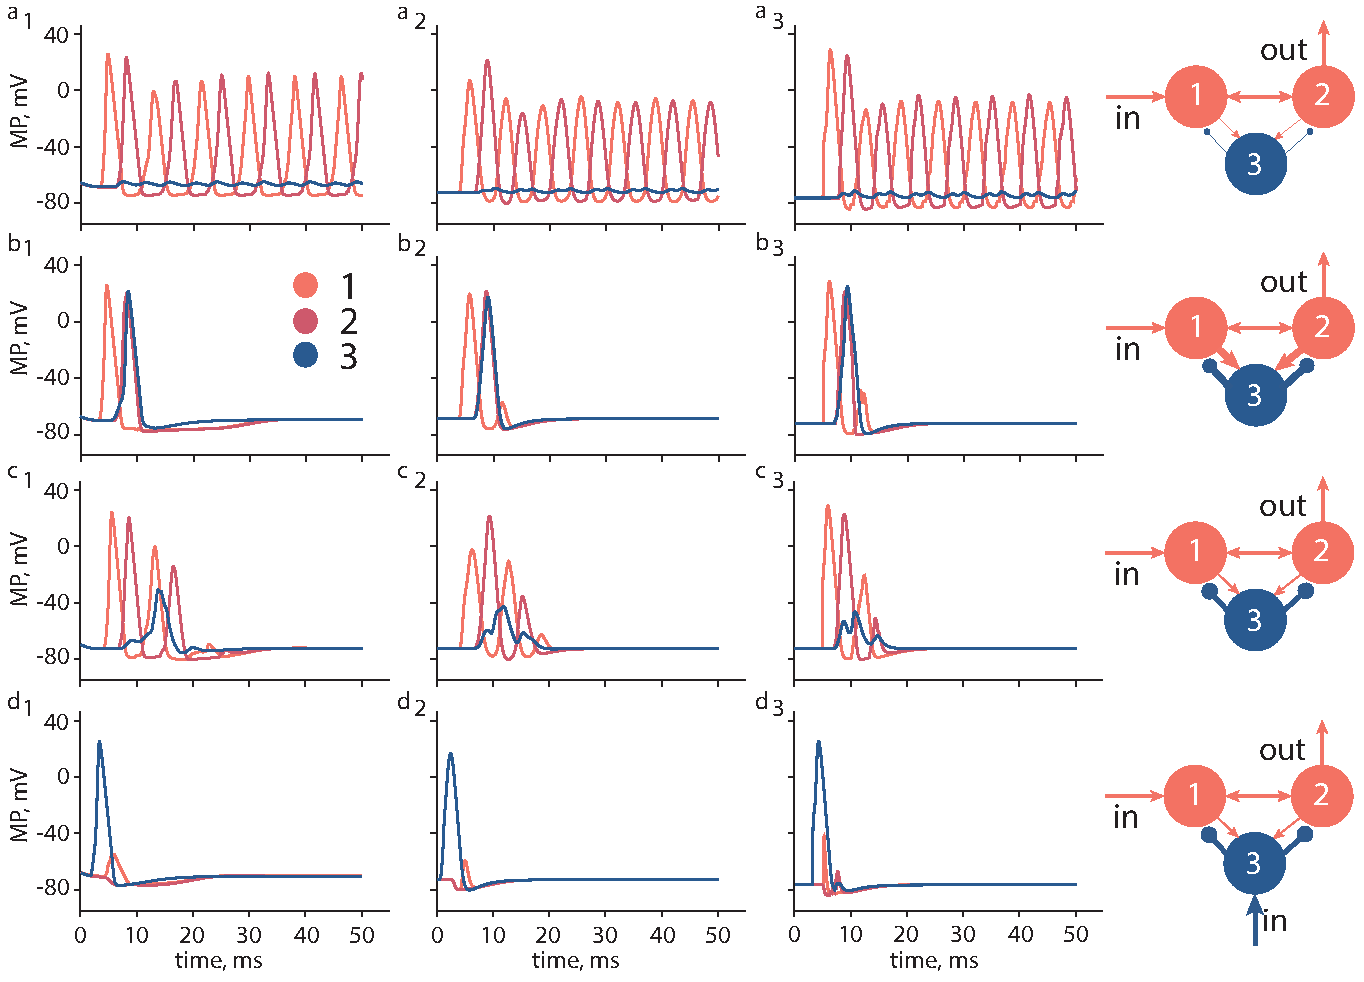
\includegraphics[width=0.8\linewidth]{OM_sim}
  \end{figure}
\end{frame}
%------------------------------------------------
%------------------------------------------------
\section{Memristive neuron}
%------------------------------------------------
\begin{frame}
  \frametitle{Oscillator motif}
  \begin{figure}
    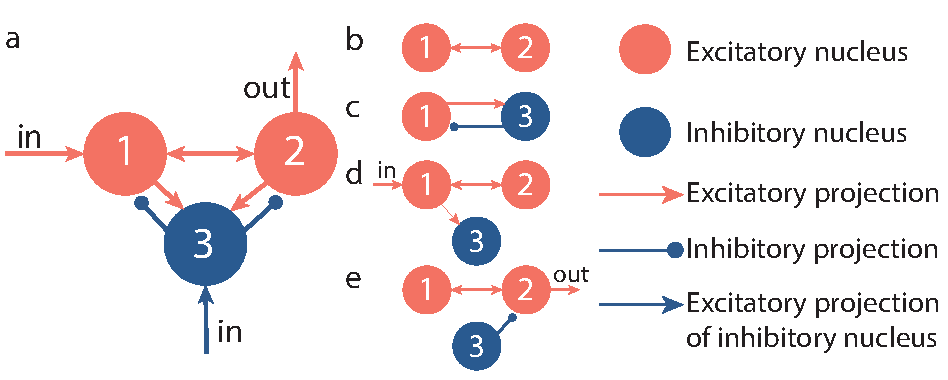
\includegraphics[width=0.8\linewidth]{OM}
  \end{figure}
\end{frame}
%------------------------------------------------




\begin{frame}
  \frametitle{Memristive spinal cord parameters}
\begin{columns}[c]
\column{.6\textwidth} % Left column and width

\emph{Reflex arc:}\\
1754 neurons, 478 200 synapses,\\
Motor neuron - 400 synapses,\\
Ia interneuron - 300,
Ib interneuron - 200,\\
Renshaw - 200,
Afferents - 100\\


\emph{CPG:}\\
880 interneurons including interneuronal pool,
40 000 synapses,
each nucleaus 20 neurons

\column{.4\textwidth} % Right column and width
\begin{figure}
\includegraphics[width=1.0\linewidth]{mousebrainpink}
\end{figure}
\end{columns}
\end{frame}

%------------------------------------------------

\end{document} 
